\chapter{Popular CNN Models}

\section{LeNet/ LeNet-5 (1998) \cite{gfg-convolutional-neural-network-cnn-in-machine-learning,wiki-lenet,ieee/726791/cnn-lenet,medium/lenet-5-complete-architecture-84c6d08215f9}}\label{cnn: LeNet}

\begin{figure}[h]
    \centering
    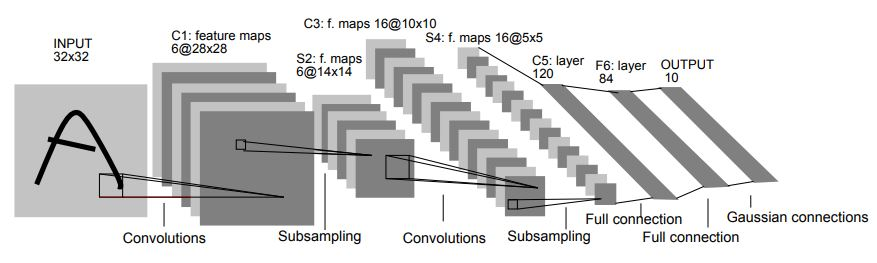
\includegraphics[width=\linewidth, height=5cm, keepaspectratio]{Pictures/convolutional-neural-network/LeNet_Original_Image.jpg}
    \caption{CNN: LeNet}
\end{figure}

\begin{itemize}
    \item LeNet is a convolutional neural network structure proposed by LeCun et al. in 1998. \cite{ieee/726791/cnn-lenet}
    
    
    \item In general, LeNet refers to LeNet-5 and is a simple convolutional neural network.
\end{itemize}


\begin{longtable}{|>{\centering\arraybackslash}m{1.5cm}|>{\centering\arraybackslash}m{2cm}|>{\centering\arraybackslash}m{1.5cm}|>{\centering\arraybackslash}c|>{\centering\arraybackslash}m{1cm}|>{\centering\arraybackslash}m{1.5cm}|>{\centering\arraybackslash}m{2cm}|>{\centering\arraybackslash}m{2cm}|}
    \caption{CNN: LeNet-5 Architecture \cite{medium/lenet-5-complete-architecture-84c6d08215f9}}\\

    \hline
    \textbf{Layer No.} & \textbf{Layer} & \textbf{Feature Map} & \textbf{Size} & \textbf{Kernel Size} & \textbf{Stride} & \textbf{Activation} & \textbf{Trainable Params} \\
    \hline
    \endfirsthead

    \hline
    \textbf{Layer No.} & \textbf{Layer} & \textbf{Feature Map} & \textbf{Size} & \textbf{Kernel Size} & \textbf{Stride} & \textbf{Activation} & \textbf{Trainable Params} \\
    \hline
    \endhead

    \hline\endfoot
    \hline\endlastfoot

    Input & Image & 1 & $32\times 32$ & - & - & - & - \\
    \hline

    1 & Convolution & 6 & $28\times 28$ & $5\times 5$ & 1 & tanh & 156 \\
    \hline

    2 & Average Pooling & 6 & $14\times 14$ & $2\times 2$ & 2 & tanh & 0 \\
    \hline

    3 & Convolution & 16 & $10\times 10$ & $5\times 5$ & 1 & tanh & 2416 \\
    \hline

    4 & Average Pooling & 16 & $5\times 5$ & $2\times 2$ & 2 & tanh & 0 \\
    \hline

    5 & Convolution & 120 & $1\times 1$ & $5\times 5$ & 1 & tanh & 48120 \\
    \hline

    6 & FC & - & 84 & - & - & tanh & 10044 \\
    \hline

    Output & FC & - & 10 & - & - & softmax & 850 \\
    \hline
\end{longtable}


\begin{lstlisting}[language=Python,caption=LeNet - tensorflow - Python]
import tensorflow as tf
from tensorflow.keras import layers, models

# Define the model
model = models.Sequential()

# Layer 1: Convolutional Layer
model.add(
    layers.Conv2D(6, (5, 5), 
    activation='tanh', 
    input_shape=(32, 32, 1))
)

# Layer 2: Average Pooling
model.add(layers.AveragePooling2D((2, 2)))

# Layer 3: Convolutional Layer
model.add(layers.Conv2D(16, (5, 5), activation='tanh'))

# Layer 4: Average Pooling
model.add(layers.AveragePooling2D((2, 2)))

# Layer 5: Convolutional Layer
model.add(layers.Conv2D(120, (5, 5), activation='tanh'))

# Flatten the tensor
model.add(layers.Flatten())

# Layer 6: Fully Connected Layer
model.add(layers.Dense(84, activation='tanh'))

# Output Layer: Fully Connected Layer
model.add(layers.Dense(10, activation='softmax'))

# Print the model summary
model.summary()
\end{lstlisting}

\textbf{Output}:
\begin{lstlisting}[numbers=none]
Model: "sequential"
_________________________________________________________________
 Layer (type)                Output Shape              Param #   
=================================================================
 conv2d (Conv2D)             (None, 28, 28, 6)         156
 average_pooling2d (Average  (None, 14, 14, 6)         0
 Pooling2D)
 conv2d_1 (Conv2D)           (None, 10, 10, 16)        2416
 average_pooling2d_1 (Avera  (None, 5, 5, 16)          0
 gePooling2D)
 conv2d_2 (Conv2D)           (None, 1, 1, 120)         48120
 flatten (Flatten)           (None, 120)               0
 dense (Dense)               (None, 84)                10164
 dense_1 (Dense)             (None, 10)                850
=================================================================
Total params: 61706 (241.04 KB)
Trainable params: 61706 (241.04 KB)
Non-trainable params: 0 (0.00 Byte)
_________________________________________________________________
\end{lstlisting}


\section{AlexNet (2012) \cite{gfg-convolutional-neural-network-cnn-in-machine-learning, medium/@siddheshb008/alexnet-architecture-explained-b6240c528bd5,wiki-AlexNet}}\label{cnn: AlexNet}

\begin{figure}[h]
    \centering
    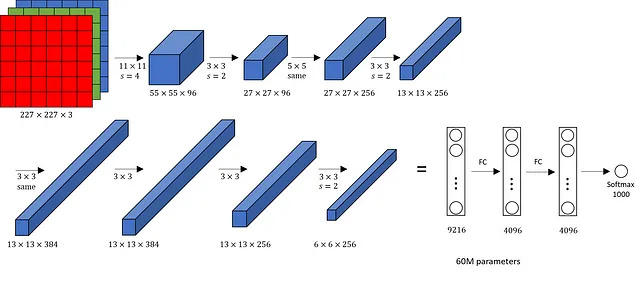
\includegraphics[width=\linewidth, height=5cm, keepaspectratio]{Pictures/convolutional-neural-network/alexnet.jpg}
    \caption{CNN: AlexNet \cite{medium/@siddheshb008/alexnet-architecture-explained-b6240c528bd5}}
\end{figure}

\begin{itemize}
    \item AlexNet is the name of a convolutional neural network (CNN) architecture, designed by \textbf{Alex Krizhevsky} in collaboration with Ilya Sutskever and Geoffrey Hinton, who was Krizhevsky's Ph.D. advisor at the \textbf{University of Toronto}. \cite{wiki-AlexNet}

    \item This was the first architecture that used GPU to boost the training performance.

    \item Architecture:\\
    \(
      \displaystyle (\text{CNN} \to \text{RN} \to \text{MP})^{2}\to (\text{CNN}^{3} \to \text{MP})\to (\text{FC} \to \text{DO})^{2} \to \text{Linear}\to \text{softmax}  \hfill \text{\cite{wiki-AlexNet}}
    \)

    \begin{table}[h]
        \centering
        \begin{tabular}{l l}
            \textbf{Layer} & \textbf{Description} \\ \hline
            CNN & convolutional layer (with ReLU activation) \\
            RN & local response normalization \\
            MP & maxpooling (SEE: \fullref{cnn: Max Pooling}) \\
            FC & fully connected layer (with ReLU activation) \\
            Linear & fully connected layer (without activation) \\
            DO & dropout \\
        \end{tabular}
    \end{table}
\end{itemize}

\begin{lstlisting}[language=Python,caption=AlexNet - tensorflow - Python]
import tensorflow as tf
from tensorflow.keras import layers, models

model = models.Sequential()

# 1st Convolutional Layer
model.add(layers.Conv2D(96, (11, 11), strides=4, activation='relu', 
        input_shape=(227, 227, 3)))
model.add(layers.MaxPooling2D((3, 3), strides=2))

# 2nd Convolutional Layer
model.add(layers.Conv2D(256, (5, 5), padding='same', activation='relu'))
model.add(layers.MaxPooling2D((3, 3), strides=2))

# 3rd Convolutional Layer
model.add(layers.Conv2D(384, (3, 3), padding='same', activation='relu'))

# 4th Convolutional Layer
model.add(layers.Conv2D(384, (3, 3), padding='same', activation='relu'))

# 5th Convolutional Layer
model.add(layers.Conv2D(256, (3, 3), padding='same', activation='relu'))
model.add(layers.MaxPooling2D((3, 3), strides=2))

# Flatten
model.add(layers.Flatten())

# 1st Fully Connected Layer
model.add(layers.Dense(4096, activation='relu'))
model.add(layers.Dropout(0.5))

# 2nd Fully Connected Layer
model.add(layers.Dense(4096, activation='relu'))
model.add(layers.Dropout(0.5))

# Output Layer
model.add(layers.Dense(1000, activation='softmax'))

# Print the model summary
model.summary()
\end{lstlisting}

\textbf{Output}:

\begin{lstlisting}[numbers=none]
Model: "sequential"
_________________________________________________________________
 Layer (type)                Output Shape              Param #   
=================================================================
 conv2d (Conv2D)             (None, 55, 55, 96)        34944     
 max_pooling2d (MaxPooling2  (None, 27, 27, 96)        0         
 D)                                                              
 conv2d_1 (Conv2D)           (None, 27, 27, 256)       614656    
 max_pooling2d_1 (MaxPoolin  (None, 13, 13, 256)       0         
 g2D)                                                            
 conv2d_2 (Conv2D)           (None, 13, 13, 384)       885120    
 conv2d_3 (Conv2D)           (None, 13, 13, 384)       1327488   
 conv2d_4 (Conv2D)           (None, 13, 13, 256)       884992    
 max_pooling2d_2 (MaxPoolin  (None, 6, 6, 256)         0         
 g2D)                                                            
 flatten (Flatten)           (None, 9216)              0         
 dense (Dense)               (None, 4096)              37752832  
 dropout (Dropout)           (None, 4096)              0         
 dense_1 (Dense)             (None, 4096)              16781312  
 dropout_1 (Dropout)         (None, 4096)              0         
 dense_2 (Dense)             (None, 1000)              4097000   
=================================================================
Total params: 62378344 (237.95 MB)
Trainable params: 62378344 (237.95 MB)
Non-trainable params: 0 (0.00 Byte)
_________________________________________________________________
\end{lstlisting}


\section{VGG-16 (2014) \cite{gfg-convolutional-neural-network-cnn-in-machine-learning,arxiv-1409.1556,gfg-vgg-16-cnn-model}}\label{cnn: VGG-16}

\begin{figure}[h]
    \centering
    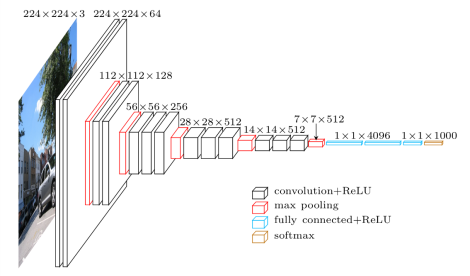
\includegraphics[width=\linewidth, height=7cm, keepaspectratio]{Pictures/convolutional-neural-network/vgg-16-1.png}
    \caption{VGG-16: Architecture - Visual}
\end{figure}
\begin{figure}[h]
    \centering
    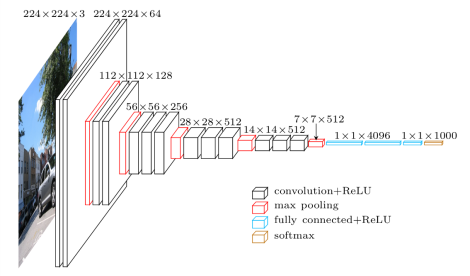
\includegraphics[width=\linewidth, height=2.5cm, keepaspectratio]{Pictures/convolutional-neural-network/vgg-16-1.png}
    \caption{VGG-16: Architecture - Visual}
\end{figure}

\begin{itemize}
    \item The VGG-16 model is a convolutional neural network (CNN) architecture that was proposed by the \textbf{Visual Geometry Group (VGG)} at the \textbf{University of Oxford}.
\end{itemize}

\begin{lstlisting}[language=Python,caption=VGG-16 - tensorflow - Python]
import tensorflow as tf
from tensorflow.keras import layers, models

model = models.Sequential()

# Block 1
model.add(layers.Conv2D(64, (3, 3), padding='same', activation='relu', 
            input_shape=(224, 224, 3)))
model.add(layers.Conv2D(64, (3, 3), padding='same', activation='relu'))
model.add(layers.MaxPooling2D((2, 2), strides=(2, 2)))

# Block 2
model.add(layers.Conv2D(128, (3, 3), padding='same', activation='relu'))
model.add(layers.Conv2D(128, (3, 3), padding='same', activation='relu'))
model.add(layers.MaxPooling2D((2, 2), strides=(2, 2)))

# Block 3
model.add(layers.Conv2D(256, (3, 3), padding='same', activation='relu'))
model.add(layers.Conv2D(256, (3, 3), padding='same', activation='relu'))
model.add(layers.Conv2D(256, (3, 3), padding='same', activation='relu'))
model.add(layers.MaxPooling2D((2, 2), strides=(2, 2)))

# Block 4
model.add(layers.Conv2D(512, (3, 3), padding='same', activation='relu'))
model.add(layers.Conv2D(512, (3, 3), padding='same', activation='relu'))
model.add(layers.Conv2D(512, (3, 3), padding='same', activation='relu'))
model.add(layers.MaxPooling2D((2, 2), strides=(2, 2)))

# Block 5
model.add(layers.Conv2D(512, (3, 3), padding='same', activation='relu'))
model.add(layers.Conv2D(512, (3, 3), padding='same', activation='relu'))
model.add(layers.Conv2D(512, (3, 3), padding='same', activation='relu'))
model.add(layers.MaxPooling2D((2, 2), strides=(2, 2)))

# Fully connected layers
model.add(layers.Flatten())
model.add(layers.Dense(4096, activation='relu'))
model.add(layers.Dropout(0.5))
model.add(layers.Dense(4096, activation='relu'))
model.add(layers.Dropout(0.5))
model.add(layers.Dense(1000, activation='softmax'))


model.summary()
\end{lstlisting}

\begin{lstlisting}[numbers=none]
Model: "sequential"
_________________________________________________________________
 Layer (type)                Output Shape              Param #   
=================================================================
 conv2d (Conv2D)             (None, 224, 224, 64)      1792      
 conv2d_1 (Conv2D)           (None, 224, 224, 64)      36928     
 max_pooling2d (MaxPooling2  (None, 112, 112, 64)      0         
 D)                                                              
 conv2d_2 (Conv2D)           (None, 112, 112, 128)     73856     
 conv2d_3 (Conv2D)           (None, 112, 112, 128)     147584    
 max_pooling2d_1 (MaxPoolin  (None, 56, 56, 128)       0         
 g2D)                                                            
 conv2d_4 (Conv2D)           (None, 56, 56, 256)       295168    
 conv2d_5 (Conv2D)           (None, 56, 56, 256)       590080    
 conv2d_6 (Conv2D)           (None, 56, 56, 256)       590080    
 max_pooling2d_2 (MaxPoolin  (None, 28, 28, 256)       0         
 g2D)                                                            
 conv2d_7 (Conv2D)           (None, 28, 28, 512)       1180160   
 conv2d_8 (Conv2D)           (None, 28, 28, 512)       2359808   
 conv2d_9 (Conv2D)           (None, 28, 28, 512)       2359808   
 max_pooling2d_3 (MaxPoolin  (None, 14, 14, 512)       0         
 g2D)                                                            
 conv2d_10 (Conv2D)          (None, 14, 14, 512)       2359808   
 conv2d_11 (Conv2D)          (None, 14, 14, 512)       2359808   
 conv2d_12 (Conv2D)          (None, 14, 14, 512)       2359808   
 max_pooling2d_4 (MaxPoolin  (None, 7, 7, 512)         0         
 g2D)
 flatten (Flatten)           (None, 25088)             0         
 dense (Dense)               (None, 4096)              102764544 
 dropout (Dropout)           (None, 4096)              0         
 dense_1 (Dense)             (None, 4096)              16781312  
 dropout_1 (Dropout)         (None, 4096)              0         
 dense_2 (Dense)             (None, 1000)              4097000   
=================================================================
Total params: 138357544 (527.79 MB)
Trainable params: 138357544 (527.79 MB)
Non-trainable params: 0 (0.00 Byte)
_________________________________________________________________
\end{lstlisting}

















































